\subsection{Dependency Probing (RQ4)}
\label{sec:rq4}

\begin{figure}[t]
 	\centering
 	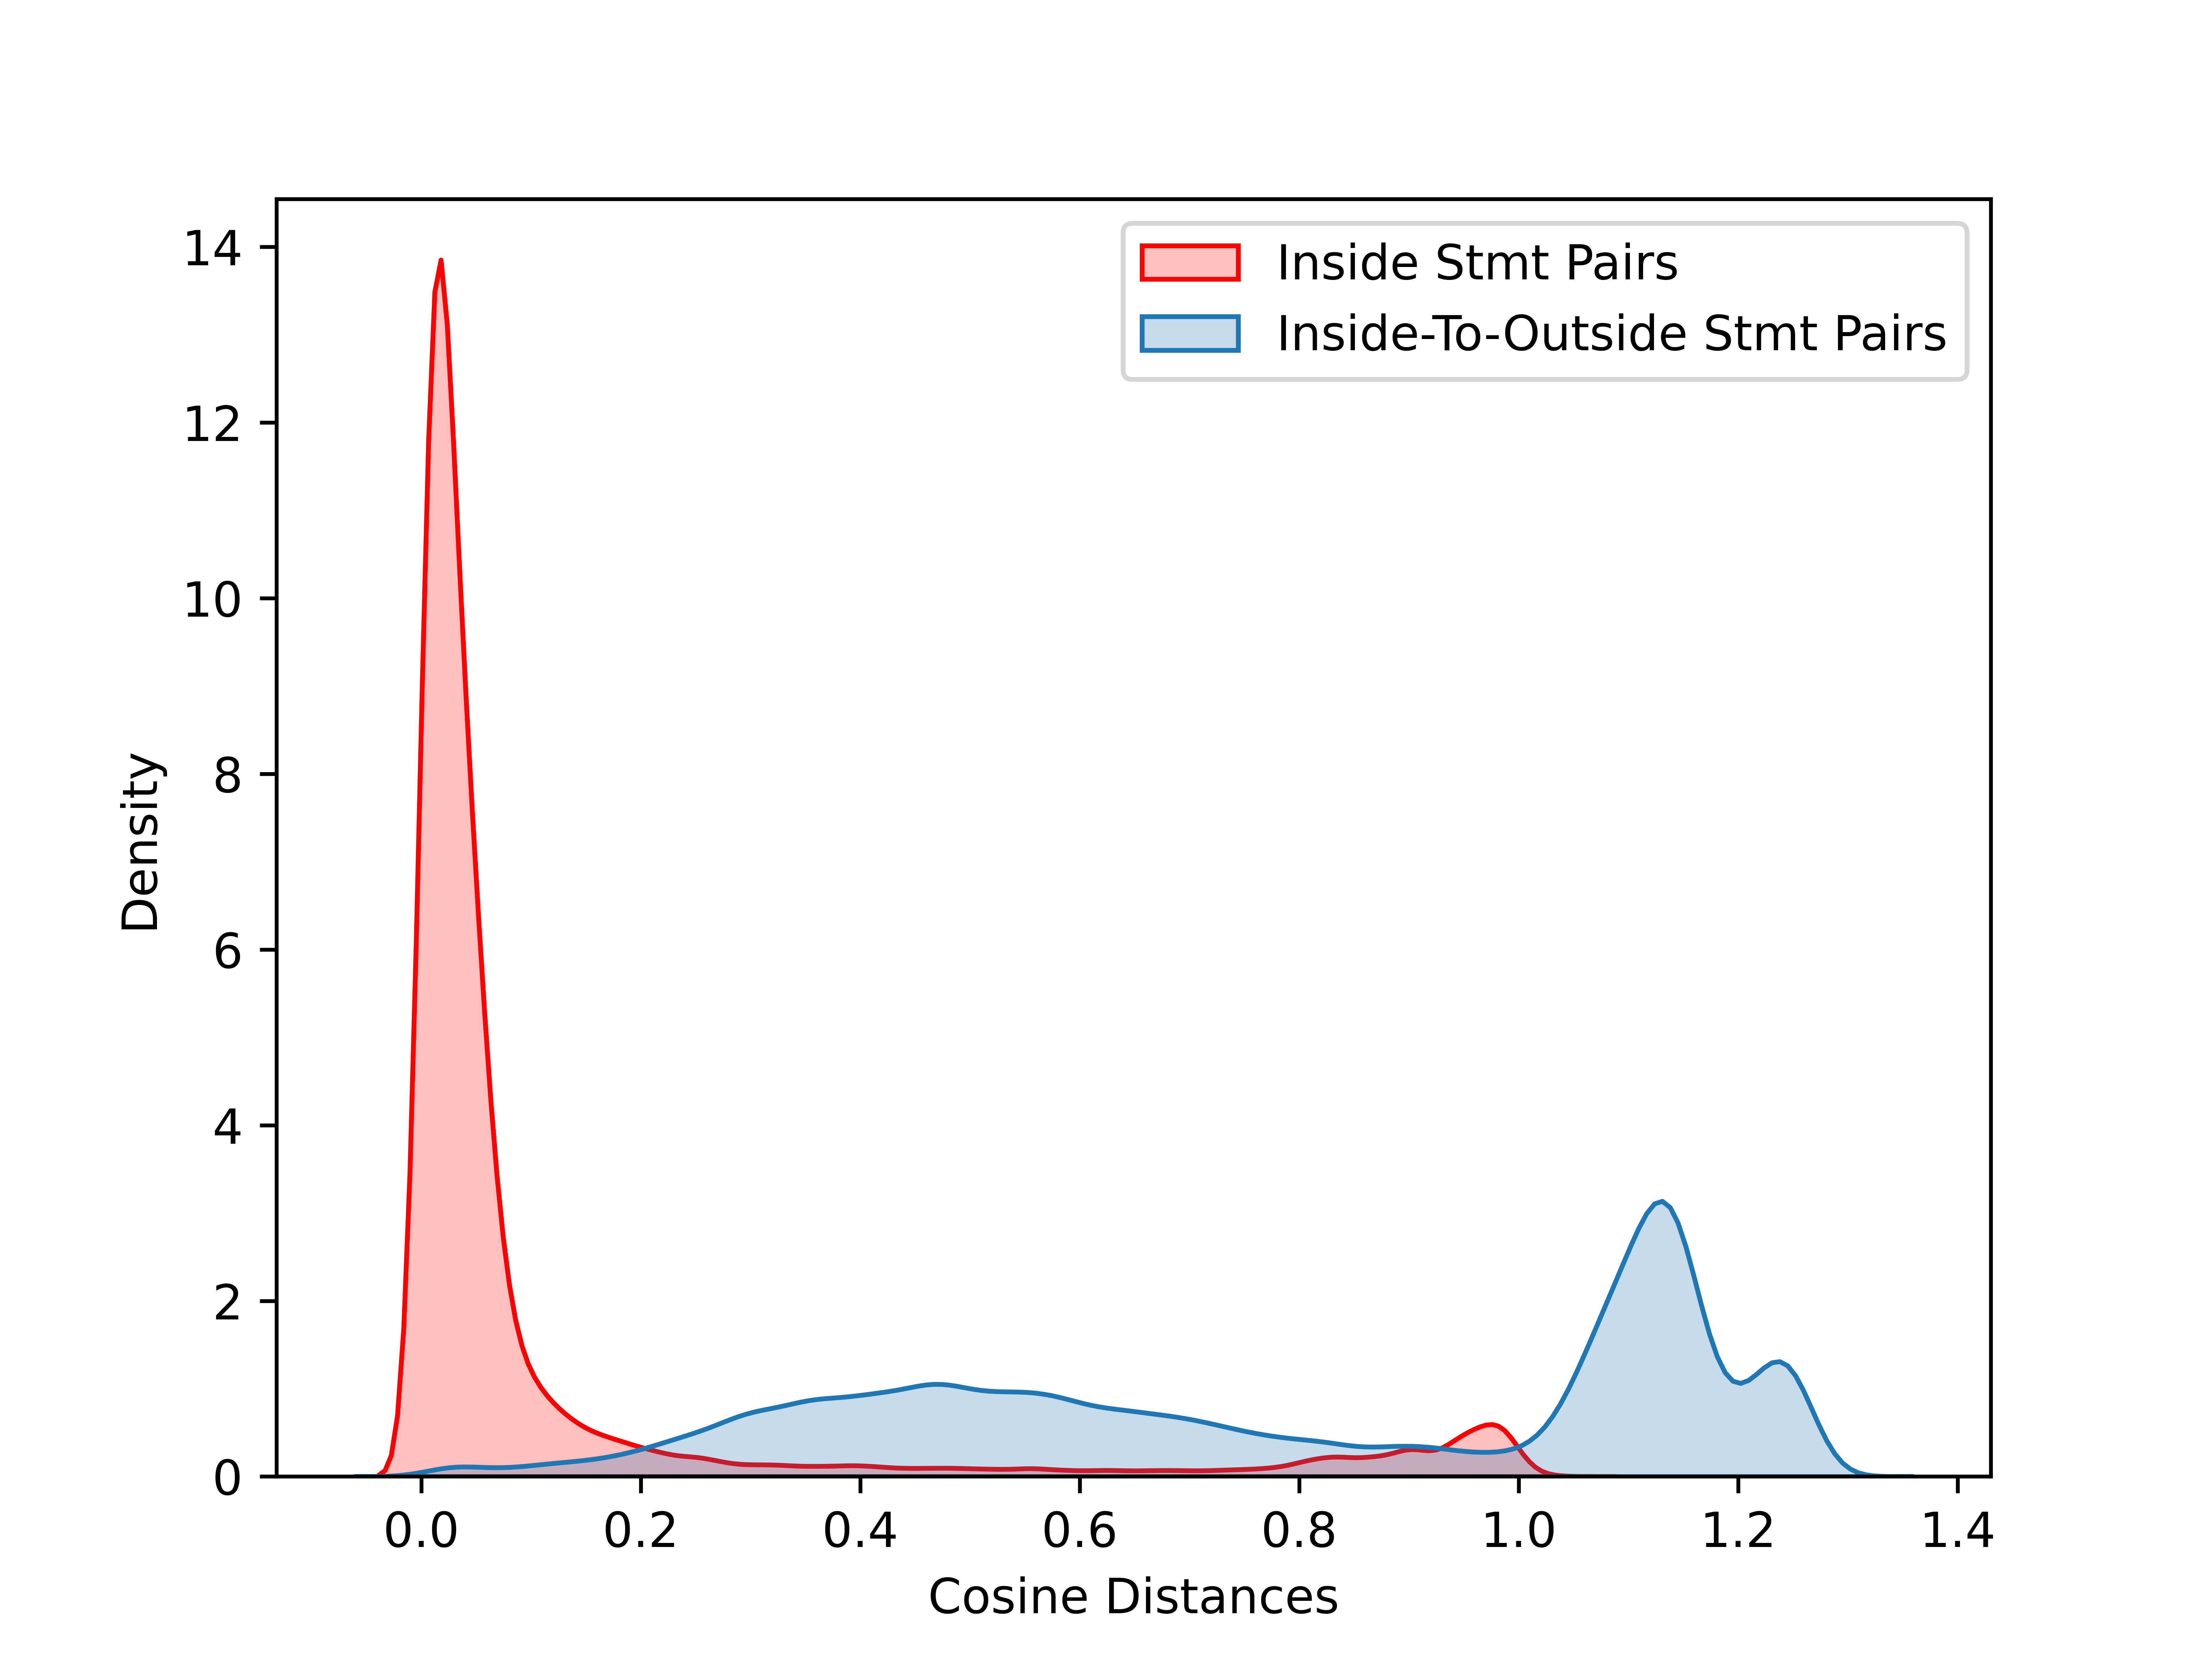
\includegraphics[width=3.4in]{rq4-density.png}
        \vspace{-20pt}
 	\caption{The Distribution of Cosine Distances broken down by Statement Groups}
 	\label{fig:rq4-density}	
\end{figure}

As seen in Figure~\ref{fig:rq4-density}, the distribution in terms of cosine distances for all the inside-to-outside statement pairs is largely to the right of the distribution for all the inside statement pairs, showing that {\tool} tends to encode statements in a way that statements in the same try block are closer to each other in the embedding space. 

The confidence interval of the mean of cosine distances for the inside statement group is 0.1262 to 0.1268 with 95\% confidence, and the confidence interval for the inside-to-outside statement group is 0.7987 to 0.8001 with 95\% confidence.